Este guia sintetiza os conhecimentos necessários para trabalhar
com o serviço LDAP v3 no barramento de serviços ERLANGMS.

O serviço LDAP v3 refere-se a implementação protocolo
Lightweight Directory Access Protocol, ou LDAP, no barramento de serviços.
O LDAP é um protocolo de aplicação aberto, livre de fornecedor e 
padrão de indústria para ser utilizado para oferecer
um "logon único" onde uma senha para um usuário é compartilhada entre muitos serviços.

O barramento de serviços ERLANGMS foi desenvolvido por Everton de Vargas Agilar
no Mestrado Profissional em Computação Aplicada da UnB com 
o intuíto de facilitar a criação e a integração de sistemas 
através de uma abordagem orientada a serviços no estilo 
arquitetural REST (Representational State Transfer). 
No entanto, outros protocolos foram adicionados para suprir tal necessidade,
entre eles, um serviço de autenticação de usuários através do protoloco LDAP.

No restante desta introdução, serão apresentados os principais 
elementos de tempo de execução do barramento de serviços ERLANGMS, 
para que o leitor possa ter uma visão geral do funcionamento
do software antes de proseguir com a instalação e configuração.


\section{Componentes em Tempo de Execução}

Os principais componentes da arquitetura do barramento de serviços 
ERLANGMS de tempo de execução 
estão listados a seguir com uma breve descrição sobre o seu objetivo
sem entrar em muitos detalhes:


\subsection{Barramento de serviços (ems-bus)}

É o software do servidor. Sua função é interligar os clientes (tipicamente os Front-ends) 
aos serviços que contém as regras de negócios da organização (como o logon do usuário). 
Quando alguém faz uma requisição para um serviço, é o software do barramento 
que intermedia o envio e o recebimento das mensagens, sendo que o cliente
só precisa saber o endereço do barramento e o protocolo utilizado. A 
Figura \ref{fig:roteamento_mensagens} mostra o esquema típico de
roteamento de mensagens HTTP/REST. Este esquem é em tudo semelhante
para o protocolo LDAP também.

\begin{figure}[htb]
\centering
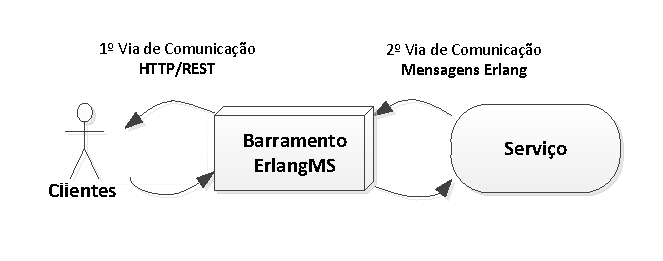
\includegraphics[scale=1.2]{/img/arquitetura/roteamento_mensagens.pdf}
\caption{Esquema do roteamento das mensagens da arquitetura.}
\label{fig:roteamento_mensagens}
\end{figure}
\FloatBarrier


\subsection{Catálogo de serviços}

Representa o componente chave da arquitetura do barramento de serviços pois permite
dar visibilidade aos serviços disponibilizados na organização. É no catálogo que 
os serviços são descritos e registrados. O exemplo a seguir expõem um serviço no catálogo 
para o serviço LDAP v3 utilizado na integração do software Redmine 
ao banco de dados de usuários SCA da UnB.


\lstset{
        basicstyle=\footnotesize,
        numbers=left,
        numberstyle=\footnotesize,
        tabsize=2,
        numbers=none,
        rulesepcolor=\color{blue}}
\renewcommand{\lstlistingname}{Código}             
\begin{lstlisting}[caption=Exemplo de um serviço no catálogo de serviços., label=fig:catalogo_processo] 
{
	"name": "ems_ldap_server",
	"comment": "LDAP service for client integration to the SCA database",
	"owner": "emsbus",
	"version": "1.0.0",
	"service" : "ems_ldap_server:start",
	"url": "/emsbus/ems_ldap_server",
	"type": "KERNEL",
	"lang" : "erlang",
	"tcp_listen_address" : ["0.0.0.0"],
	"tcp_allowed_address" : ["*.*.*.*"],
	"tcp_port": 2389,
	"datasource" : {
		"type" : "sqlserver",
		"connection" : "string conection",
		"primary_key" : "PesCodigoPessoa",
		"timeout" : 3000,
		"max_pool_size" : 10
	},	
	"ldap_admin" : "cn=admin,dc=unb,dc=br",
	"ldap_password_admin" : "xxxxxxxxx",
}
\end{lstlisting}


\subsection{Módulo Back-end}

O Back-end é a implementação dos serviços. Tipicamente
os serviços são implementados na linguagem Java no CPD/UnB
mas podem ser desenvolvidos em qualquer linguagem que possua 
o SDK do barramento de serviços. 


\subsection{Módulo Front-end}

Consiste na interface da aplicação bem como a parte que o usuário vê. O front-end é o responsável por coletar os dados de entrada do usuário
e realizar as chamadas para os serviços por meio do barramento de serviços.

\subsection{Servidor de Aplicação JBoss/Wildfly}

O servidor de aplicação JBoss/Wildfly é onde são publicados (deployment)
os projetos Java Web. Podem existir várias instâncias desses servidores para
aumentar a escalabilidade dos serviços, sendo que o barramento despacha
as requisições dos clientes utilizando um simples algoritmo round-robin.

\subsection{Erlang Port Mapper Daemon}

É um serviço que executa em 
segundo plano em cada nó de um cluster e que age como um servidor de nome.
É importante salientar que tanto o barramento quanto os
servidores de aplicação JBoss/Wildfly são vistos como nós 
na arquitetura. O cliente não faz parte do cluster pois é apenas um consumidor.

